\section{Stage 3: Full Payload Recovery}
Stage 2 in the previous section uses the braking valve B2 to reduce the rate of cable loss $\dot{\psi}r_W$ until $\dot{\psi}r_W = 0$. At this point, stage 3 is initiated to make a full recovery of the payload and all lost cable. 

When stage 3 is initiated, the 4 way, 2 position valve is put into position I. Figure \ref{fig:WINCH_HYDRAULICS_DIAGRAM_VP1} illustrates the valve position change from II to I. This allows the variable displacement, pressure compensated pump to push hydraulic fluid in the the H node, increase the pressure, and apply torque to the fixed displacement hydraulic motor to pull in the payload. Once this occurs, the $P_{set}$ value in eq. \ref{eq:D_PII} relisted below is set to $P_{set} = 15\hspace{1mm}psi$ \cite{MathWorks2015bb}.
\begin{equation*}
D_P = \left\{
        \begin{array}{ll}
            D_{P,Max} & \quad P_H \leq P_{set} \\
            D_{P,Max} - k_P(P_H - P_{set}) & \quad P_{set} < P_H < P_{Max} \\
            0 & \quad P_H \geq P_{Max}
        \end{array}
    \right.
\end{equation*}
This small initial $P_{set}$ value is used since $P_H = 0\hspace{1mm}psi$ at the instant the valve position change occurs and the variable displacment, pressure compensated pump model puts the pump to its maximum displacement value $D_{P,Max}$ if $P_H \leq P_{set}$. This minimizes the amount of time the pump fully loads the engine to provide a stable transition and to not stall out the tractor's engine.
\begin{figure}[ht]
    \centering
    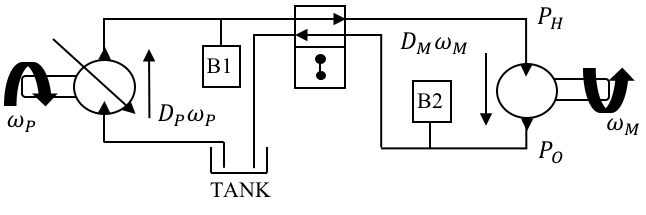
\includegraphics[width = 4in, keepaspectratio]{WINCH_HYDRAULICS_DIAGRAM_VP1}
    \caption{Diagram of the winch hydraulic system in stage 3 of the winch control mode. The 4 position 2 way valve is shifted from position II to position I. This allows a build up of pressure in the H node of the hydraulic system to increase the torque applied the fixed displacement hydraulic motor and subsequently the winch.}
    \label{fig:WINCH_HYDRAULICS_DIAGRAM_VP1}
\end{figure}
After the initial transition, the winch follows a similar procedure to Algorithm \ref{alg:WIPC}. This brief rule based procedure is summarized in algorithm \ref{alg:WIFR} and is identical to to the procedure used in stage 2 but omits the cautionary step of greatly reducing drawbar pull if the vehicle detects $\hat{i} \geq 35\%$. There are several reasons for this. First, if the tractor has progressed from stage 2 to stage 3, the immediate terrain will provide enough traction to reel in the payload. Second, if the tractor is not able to recover the entire length of the cable due to another immediate soft terrain encounter, it is likely that the soft terrain patches that occur in the operating environment are too frequent and/or to long. Third, the drawbar requirements in the 3rd stage are slightly different than in the 2nd stage. In the 2nd stage, the winch is attempting to bring the speed of the winch $\dot\psi r_W$ to zero. Therefore, to make progress, the second derivative $\ddot\psi r_W$ must always be non-zero or negative in this case to make progress. This acceleration requires a drawbar load constantly in excess of what is required to pull the payload in order to complete the 2nd stage.
\begin{algorithm}[hb]
\setstretch{1.35}
\SetAlgoLined
\vspace{5pt}
 $incPSI = 15\hspace{1mm}psi$\;
 \If{winch control mode is active and 4 way, 2 position valve is in position I}{
  $\hat{i}\leftarrow$ last slip estimate from DTKF\;
  \uIf{$\hat{i} \leq 20\%$}{
   $P_{set} = P_{set} + incPSI$\;
   }
  \ElseIf{$ i > 20\%  $}{
  maintain current $P_{set}$\;
  }
 }
 \caption{Winch Full Payload Recovery (4 Hz)}\label{alg:WIFR}
\end{algorithm}
However in stage 3, a constant winch speed results in progress towards full recovery of the payload. Therefore, additional drawbar load in excess of what is required to tow the payload or a nonzero value of $\ddot\psi r_W$ is only needed briefly instead of constantly as in stage 2.